\documentclass[12pt,twoside]{report}
\usepackage[a4paper,width=150mm,top=25mm,bottom=25mm]{geometry}
\usepackage[utf8]{inputenc}     % for éô
\usepackage[english]{babel}     % for proper word breaking at line ends
\usepackage{graphicx}           % for ?
\usepackage{amsmath,amssymb}    % for better equations
\usepackage{amsthm}             % for better theorem styles
\usepackage{mathtools}          % for greek math symbol formatting
\usepackage{enumitem}           % for control of 'enumerate' numbering
\usepackage{listings}           % for control of 'itemize' spacing
\usepackage{todonotes}          % for clear TODO notes
\usepackage{hyperref}           % page numbers and '\ref's become clickable
\usepackage{ dsfont }
\usepackage{ stmaryrd }
\usepackage{float} 
\usepackage{tikz}
\usepackage{algorithm}
\usepackage{caption}
\usepackage{subcaption}
\usepackage[noend]{algpseudocode}
\graphicspath{{D:/Thesis/img/}}
\usetikzlibrary{automata, positioning, arrows}

\newcommand{\algorithmref}[1]{Algorithm~\ref{#1}}
\newcommand{\figureref}[1]{Figure~\ref{#1}}
\newcommand{\defref}[1]{Definition~\ref{#1}}
\newcommand{\lineref}[1]{Line~\ref{#1}}

\newcommand{\code}[1]{\texttt{#1}}



%%%%%%%%%%%%%%%%%%%%%%%

\begin{document}
	\begin{titlepage}
		\thispagestyle{empty}
		\newcommand{\HRule}{\rule{\linewidth}{0.5mm}}
		\center
		\textsc{\Large Radboud University Nijmegen}\\[.7cm]
		\includegraphics[width=25mm]{img/in_dei_nomine_feliciter.eps}\\[.5cm]
		\textsc{Faculty of Science}\\[0.5cm]
		
		\HRule \\[0.4cm]
		{ \huge \bfseries \thesistitle}\\[0.1cm]
		\textsc{\thesissubtitle}\\
		\HRule \\[.5cm]
		\textsc{\large Thesis MSc Computing Science}\\[.5cm]
		
		\begin{minipage}{0.4\textwidth}
			\begin{flushleft} \large
				\emph{Author:}\\
				\thesisauthorfirst\space \textsc{\thesisauthorsecond}
			\end{flushleft}
		\end{minipage}
		~
		\begin{minipage}{0.4\textwidth}
			\begin{flushright} \large
				\emph{Supervisor:} \\
				\thesissupervisorfirst\space \textsc{\thesissupervisorsecond} \\[1em]
				\emph{Second reader:} \\
				\thesissecondreaderfirst\space \textsc{\thesissecondreadersecond}
			\end{flushright}
		\end{minipage}\\[4cm]
		\vfill
		{\large \thesisdate}\\
		\clearpage
	\end{titlepage}
	
	\tableofcontents
	
	\newpage
	
	\chapter*{Abstract}
	We study how to obtain reward controllers (RCs) from history-based reward functions specified for partially observable Markov decision processes (POMDPs). A history-based reward function can be specified as a number of sequences or regular expressions together with their respective rewards. We create a product of the RC and the original POMDP to obtain an induced POMDP. Then, allowing for a maximum length of the sequence, we show how to obtain a policy for obtaining the maximum expected reward for the original POMDP.
	
	\chapter{Introduction}
	In reinforced learning we are often shown models in which the agent gets a reward for certain behavior. This behavior can also include a reward that will given only after a certain time or only given a certain history. These history-based reward functions have been studies quite a lot. More specifically, a number of results have been found to obtain a policy concerning the expected optimal reward for these history-based reward functions for MDPs\cite{p:jirp}\cite{p:rdp}.\todo{talk a bit about these?}
However for POMDPs, the task of obtaining an policy that ensures the maximum reward (or minimum cost) for history-based reward functions, is computative heavy. The belief MDP representing a POMDP can be continuous, storing the history observed for sequences and not knowing how long the sequence needs to be can be memory intensive.

Removing the history-based function would remove some of this memory intensive process. For this we present so-called Reward Controllers, which are finite automata which represent the history-based reward function used for the POMDP. This reward controller can then be combined with the original POMDP, to create an induced POMDP. This induced POMDP doesn't need to store the relevant history anymore, which was necessary for the original POMDP. The new reward function is then only based on the current state and the action, allowing us to use known methods to calculate the optimal expected reward and to find a policy.


\section*{Problem Formulation}
Given a POMDP with a history-based reward function, obtain a policy that maximizes the expected reward.


\section*{Structure}
In chapter 2 we present the preliminaries. Chapter 3 portrays all relevant definitions and shows the background information used.
In chapter 4 we present the Reward Controllers and how to obtain them from a given history-based reward function. In chapter 5 we show the newly induced POMDP which is obtained from the original POMDP together with the Reward Controller that represents the related history-based reward function. 
	
	\chapter{Preliminaries}
	\section*{Set Theory}
Let $S$ be any countable set, then $|S|$ denotes the cardinality. We let $S^*$ and $S^\omega$ denote the set of finite and infinite sequences over $S$, respectively. For a sequence $\pi\in S^*$ we can denote the length by $|\pi|$.


\section*{Probability Theory}
For any countable set $S$ we can define a \textit{discrete probability distribution} as $\psi: S\to[0,1]$ where $\sum_{s\in S} \psi(s)=1$. The set of all possible probability distributions over $S$ is denoted as $\Pi(S)$. We denote the support of a \textit{probability distribution} as $supp(\psi)=\{s\in S\mid \psi(s)>0\}$.\\

\towrite{random variable, expected value}
%- expected value of a discrete random variable E[X]





	
	\chapter{Background}
	\section{Finite Automata}
\towrite{introduction to dfa}

\begin{definition}[DFA]
A Deterministic Finite Automata is a tuple $D=(Q,q_0,\Sigma,\delta,F)$ where 
\begin{itemize}
\item $Q$, the finite set of states;
\item $q_0$, the initial state;
\item $\Sigma$ the input alphabet;
\item $\delta: Q\times\Sigma\to Q$, the deterministic transition function;
\item $F\subseteq Q$, the set of final states.
\end{itemize}
\end{definition}

\towrite{introduction to lambda star}
\begin{definition}
We define $\delta^*:Q\times\Sigma^*\to Q$ where $\delta^*(q,w)$ denotes the state we end up after reading word $w$ starting from state $q$ as follows
\begin{equation*}
\delta^*(q,w)=\begin{cases}
	q &\text{if } w=\epsilon \\
	\delta^*(\delta(q,a_1),a_2\dots a_n) & \text{if } w=a_1a_2\dots a_n
	\end{cases}
\end{equation*}
\label{d:delta_star}
\end{definition}

\towrite{introduction to accepted words}

\begin{definition}
We say the language accepted by a DFA $D=(Q,q_0,\Sigma,\delta,F)$ consists of all the words that start in the begin state and finish in any final state. Thus $L(D)=\{w\in\Sigma^*\mid \delta^*(q_0,w)\in F\}$.
\label{d:accepted_language}
\end{definition}



\section{Markov decision processes}

\towrite{introduction to MDP}
\begin{definition}[MDP]
	A Markov decision process is a tuple $M=(S,s_I,A,T)$ where 
	\begin{itemize}
		\item $S$, the finite set of states;
		\item $s_I\in S$, the initial state;
		\item $A$, the finite set of actions;
		\item $T:S\times A\to \Pi(S)$, the probabilistic transition function.
	\end{itemize}
\end{definition}

Note that given $s\in S,a\in A$, we assign a probability distribution over $S$ through $T(s,a)$. To obtain the probability of ending up in a certain state $s'$ when starting in state $s$ and performing action $a$, we simply calculate $T(s,a,s')$ which we obtain through $T(s,a)(s')$.\\

The \textit{available actions} for a state $s$ are given by $A(s)=\{a\in A\mid \exists s'\in S: T(s,a,s')>0\}$. We can give the \textit{possible successors} of state $s$ in a similar matter through $Succ(s)=\{s\in S\mid\exists a\in A : T(s,a,s')>0\}$.

A finite \textit{trajectory} or \textit{run} $\pi$ of an MDP is realization of the stochastic process performed by the MDP denoted by the finite sequence $s_1 a_1 s_2 a_2\dots s_{n-1} a_{n-1} s_n \in (S\times A)^*\times S$. To obtain the last state of a trajectory we can use the following \[last(\pi)=last(s_1 a_1 s_2 a_2\dots s_{n-1} a_{n-1} s_n)=s_n\].

\subsection*{Reward function}
We can extend MDPs with a \textit{reward function} $R$ which assign a reward - usually in $\mathbb{R}$ for taking a certain action $a$ in a state $s$. 

\towrite{Intuitive explanation for reward function - including cost function, including a real-world example}

Let us look at \textit{Markovian reward functions}, which can determine a reward based on the current state, action and obtained state, independent of its history. The most conventional notation is $R:S\times A\to \mathbb{R}$, where we consider the current state and the taken action. Another possible definition is $R:S\times A\times S\to\mathbb{R}$, where  in $R(s,a,s')$ we consider the specific transition from $s$ to $s'$ by using action $a$, or $R:S\to\mathbb{R}$ where in $R(s)$ we only consider the visited state $s$. 

\towrite{Real life example of reward function with history}

A reward function which is dependent of its history is called a \textit{Non-Markovian reward function}. There are a number of different reward functions possible
\begin{itemize}
	\item $R:S^*\to\mathbb{R}$ - which only looks at the finite states visited, or;
	\item $R:(S\times A)^*\to\mathbb{R}$ - which looks at the finite (sub)trajectory without the last state, or;
	\item $R:(S\times A)^*\times S\to \mathbb{R}$ - which looks at the finite (sub)trajectory.
\end{itemize}

The reward function we will be using is the Non-Markovian reward function which looks at trajectories of specific length $k$, namely $R_k:(S\times A)^k\to\mathbb{R}$. 

\towrite{Increasing k creates increased reward}


\subsection*{Policy}
As stated above, we use reward functions over a MDP to usually argue over an optimized expected reward. After retrieving such an optimum, the question remains on how to actually obtain this value. We wish to know what strategy to apply path to take to obtain this value. For this we use strategies, or often called policies. 

\begin{definition}
	A policy for a MDP $M$ is a function $\sigma:(S\times A)^*\times S \to \Pi(A)$, which maps a trajectory $\pi$ to a probability distribution over all actions. 
\end{definition}

We call a policy \textit{memoryless} if the function only considers $last(\pi)$ in deciding the actions. 

\towrite{induced markov chain for removing non-determinism}

\section{Partial observability}
\towrite{Introduce pomdp}

\begin{definition}[POMDP]
	A partially observable Markov decision process (POMDP) is a tuple $\mathcal{M}=(M, \Omega, O)$ where 
	\begin{itemize}
		\item $M=(S,s_I,A,T)$, the hidden MDP;
		\item $\Omega$, the finite set of observations;
		\item $O:S\to \Omega$, the observation function. %or use O: S x A -> \Omega ?
	\end{itemize}
\end{definition}

Let $O^{-1}:\Omega\to 2^S$ be the inverse function of the observation function - $O^{-1}(o)=\{s\in \mid O(s)=o\}$ - in which we simply obtain all states in $S$ that have observation $o$.
Without loss of generality we assume that states with the same observations have the same set of available actions, thus $O(s_1)=O(s_2)\Rightarrow A(s_1)=A(s_2)$.

Since the actual states in a trajectory of the hidden MDP are not visible to the observes, we argue about an \textit{observed trajectory} of the POMDP $\mathcal{M}$. This is not consist of a sequence of states and actions, but instead a sequence of observations are actions, thus an element of $(\Omega\times A)^*\times \Omega$. The set of all possible finite observed trajectories of will be denoted as $ObsSeq^{\mathcal{M}}$.

We can argue about the observed trajectory through the observation function, which will be extended over trajectories, like so
\[O(\pi)=O(s_1 a_1 s_2 a_2\dots s_{n-1} a_{n-1} s_n) = O(s_1) a_1 O(s_2) a_2\dots O(s_{n-1}) a_{n-1} O(s_n)\]

\subsection*{Policy}
\begin{definition}
	An observation-based strategy of a POMDP $\mathcal{M}$ is a function $\sigma:ObsSeq^{\mathcal{M}}\to\Pi(A)$ such that $supp(\sigma(O(\pi)))\subseteq A (last(\pi))\ \forall \pi\in(S\times A)^*\times S$.
\end{definition}

\section{Belief MDP}



\section{Moore machine}
Based on the definition as presented in \cite{p:moore}.
\begin{definition}
	A Mealy machine is a tuple $(Q,q_0,\Sigma,O,\delta,\sigma)$ where
	\begin{itemize}
		\item $Q$, the finite set of states;
		\item $q_0\in Q$, the initial state;
		\item $\Sigma$, the finite set of input characters - the input alphabet;
		\item $O$, the finite set of output characters - the output alphabet;
		\item $\delta: Q\times \Sigma\to Q$, the input transition function, and;
		\item $\sigma : Q\to O$, the output transition function.
	\end{itemize}
\end{definition}
\subsection*{Example}
\towrite{example moore machine -- traditional sense}
	
	\chapter{Reward Controllers}
	\section{Definition}


\towrite{introduction}
The idea is to transform the history-based reward function into something more tangible. We transform it is so that we can obtain the reward per step instead of only at the end of a sequence.


Based on the history-based reward function $R:\Omega^*\to\mathbb{R}$ of a POMDP $\mathcal{M}$, we build a reward controller that mimics its behavior.

%todo: basically the same as a moore machine

%idea: when the word is done reading, you then obtain the reward. Normally when using a Moore machine you get the reward every time you enter it. However, since we won't be using the reward controller as a usual moore machine, it's fine to encodew it in the state. We will see in the next chapter how we then obtain the reward.

\begin{definition}
	A reward controller $\mathcal{F}$ is a reward machine $(N,n_I, \Omega, \mathbb{R}, \delta, \lambda)$, where
	\begin{itemize}
		\item $N$, the finite set of memory nodes;
		\item $n_I\in N$, the initial memory node;
		\item $\Omega$, the input alphabet;
		\item $\mathbb{R}$, the output alphabet;
		\item $\delta: N \times \Omega \to N$, the memory update;
		\item $\sigma: N \to \mathbb{R}$, the reward output. 
	\end{itemize}
\end{definition}

\towrite{transition to delta star}

\begin{definition}
We define $\delta^*:N\times\Omega^*\to N$ where $\delta^*(n,w)$ denotes the state we end up after reading word $\pi$ starting from state $n$ as follows
\begin{equation*}
\delta^*(n,\pi)=\begin{cases}
	n &\text{if } \pi=\epsilon \\
	\delta^*(\delta(n,o_1),o_2\dots o_n) & \text{if } \pi=o_1 o_2\dots o_n
	\end{cases}
\end{equation*}
\label{d:delta_star_rc}
\end{definition}


\section{From a list of sequences}
\label{sec:rc-sequences}
Let's say we are designing a model for an engineer and they want certain observation sequences to connect to a reward. Thus we are given a number of observation sequences $\texttt{seq}_1,\texttt{seq}_2,\dots,\texttt{seq}_n$ together with their associated real valued rewards $r_1,r_2,\dots,r_n$.
\begin{definition}
Given the observation sequences $\texttt{seq}_1,\texttt{seq}_2,\dots,\texttt{seq}_n$ and their associated rewards $r_1,r_2,\dots,r_n$ we define the history-based reward function $R:\Omega^*\to\mathbb{R}$, which we create as follows
\[R(w) = \begin{cases}
	r_i &\text{ if } w=\texttt{seq}_i \text { for } i\in \{1,\dots,n\} \\
	0   &\text{ otherwise}
	\end{cases}\]
	\label{d:created_reward_function}
\end{definition}
In $R$ we simply connect the observation sequence $\texttt{seq}_i$ to their respective reward $r_i$ and every other sequence is connected to zero.\\

We only want to obtain any of the rewards if their associated observation sequence has been observed in its entirety. Thus we create a reward controller in which we encode the reward in the node we end up in after reading the entire sequence. The idea is as follows: if we read the observation sequence and we end up in a certain node $n$, we obtain the reward $\sigma(n)$ in that node. It's important to note that if we, for example, have $R(\blacksquare\blacksquare)=2$ and $R(\blacksquare\blacksquare\square)=3$ and we read $\blacksquare\blacksquare\square$ we will only obtain reward $3$. 

Given all the sequences over which the Non-Markovian reward function is defined, let us create a reward controller through the following procedure. Note that we assume that all the sequences are unique.
\begin{algorithm}[H]
	\begin{algorithmic}[1]
		\Procedure{CreateRewardController}{sequences, $R$}
		\Require sequences
		\Require $R : \Omega^* \to \mathbb{R}$
		\State $n_I \gets $ \code{new Node()} \Comment{initial node} \label{l:initial_node}
		\State $n_F \gets $ \code{new Node()} \Comment{dump node}  \label{l:dump_node}
		\State \texttt{path}$(n_I)=\lambda$ \label{l:empty_path}
		\State $N\gets\{n_I,n_F\}$
		\ForAll{$\texttt{seq}=o_1 o_2\dots o_k$ in sequences}
			\State $n \gets n_I$
			\For{$i\gets 1,\dots, k$}
				\If{$\delta(n,o_i)$ is undefined}
					\State $n'\gets$ \code{new Node()} \Comment{create new memory node} \label{l:new_transition}
					\State \texttt{path}$(n)=o_1\dots o_i$
					\State $N \gets N \cup \{n'\}$		
					\State $\delta(n,o_i) \gets n'$	\label{l:set_transition}
				\EndIf 
				\State $n \gets \delta(n,o_i)$     \Comment{update memory node}
			\EndFor
			\State $\sigma(n) \gets R(\texttt{seq})$ \Comment{set reward} \label{l:set_reward}
		\EndFor
		\ForAll{$n\in N$} \Comment{makes $\delta$ and $\sigma$ deterministic}
			\ForAll{$o\in\Omega$}
				\If{$\delta(n,o)$ is undefined} \Comment{useless transition}
					\State $\delta(n,o) \gets n_F$ \label{l:self_loop}
				\EndIf
			\EndFor
			\If{$\sigma(n)$ is undefined}
				\State $\sigma(n) \gets 0$ \label{l:set_zero}
			\EndIf
		\EndFor
		\State \Return $(N,n_I,\Omega,\mathbb{R},\delta,\sigma)$
		\EndProcedure
	\end{algorithmic}
	\caption{Procedure for turning a list of sequences into a reward controller}
	\label{procedure:into_reward_controller}
\end{algorithm}

We start by creating an initial node in \lineref{l:initial_node} and a dump node in \lineref{l:dump_node}. The idea is that, since the reward controller is deterministic, if we need to determine the reward of a sequence that is (for example) longer than a known sequence (with reward), we don't want to end in the node in which the reward is encoded. Thus these zero-reward sequences are passed along to a node which will only consist of self-loops and will have a reward of zero encoded to them.

Then for every sequence which we are given, we walk through it. If we then come across a transition which isn't defined yet, we define it by making a new memory node in \lineref{l:new_transition}, adding it to $N$, and setting the transition to this new node. If the transition already existed, we simply update the memory node. After we are done with reading the sequence, we simply encode the reward into the node itself in \lineref{l:set_reward}.

Then since the reward controller needs to be deterministic, we set the other undefined values. Every other transition that hasn't been made yet, will be transferred to the dump node as mentioned above in \lineref{l:self_loop}. Furthermore, there are still nodes in which the reward is undefined. None of the given sequences ended up in these nodes, so per \defref{d:created_reward_function} we encode those to zero in \lineref{l:set_zero}.

Note that the set of nodes $N$ without $n_F$ together with the memory update function is represents a directed acyclic graph. This indicates for every node $n$ there is an unique path from the initial node $n_I$ to node $n$. This unique path is encoded in the function \texttt{path}$:N\setminus\{n_F\}\to\Omega^*$. This function is well-defined, since it's defined for $n_I$ in \lineref{l:empty_path}. Every other time a new node is neccesary, it is created in \lineref{l:new_transition}, and \texttt{path} is then immediately defined for the new node. This \texttt{path} function is needed for proving the following lemma. 


\begin{lemma}
For any sequence $\texttt{seq}\in\Omega^*$, let $r=R(\texttt{seq})$ be its associated reward. Then $\sigma(\delta^*(n_I,\texttt{seq}))=r$.
\begin{proof}
Given a sequence $\texttt{seq}$, we set $n$ to be the node we end up in, i.e. $n = \delta^*(n_I,\texttt{seq})$. \\
Now if $n=n_F$, we know that the associated reward is zero since $\sigma(n_F)=0$ per construction. A sequence can only end up in $n_F$ if it was not a part of the pre-defined sequences and following \defref{d:created_reward_function} the reward is then zero. \\
If $n\in N\setminus \{n_F\}$, we can obtain the unique path to node $n$ through $\texttt{path}(n)$. We know that this is equal to $\texttt{seq}$, so the associated reward is thus $R(\texttt{path}(n))=R(\texttt{seq})=r$.
\end{proof}
\label{lem:proof_seq}
\end{lemma}


We observe that the number of memory nodes $|N|$ of the newly created reward controller $\mathcal{F}$ is bounded by $|\Omega|^k + 1$, where $k=\max\limits_{seq\in sequences} |seq|$.\\
We acknowledge that this can lead to quite large reward controllers. Please note that using state of the art automata learning, the sizing of the reward controller obtained for a number of sequences can be decreased.

\subsection*{Example}
Say we are given the following sequences and rewards
\begin{enumerate}
	\item $\square\ \square\  $ with a reward of 15
	\item $\blacksquare\ \square\ \blacksquare\ $ with a reward of 20
	\item $\square\ \square\ \blacksquare\ \square\ $ with a reward of 12
	\item  $\blacksquare\ $ with a reward of 2
\end{enumerate}

Following the procedure~\ref{procedure:into_reward_controller} we create the associated reward controller. To show how the procedure works, we will show you the intermediate reward controller after processing every sequence. 

\subsubsection*{After sequence (1)}
\begin{figure}[H]
	\centering
		\begin{tikzpicture}[node distance=3cm,on grid,auto,shorten >=1pt,thick]
			\node[initial,state] (1) 				{$n_I$};
			\node[state] (2) [above right=of 1]		{$n_1$};
			\node[state] (3) [above right=of 2]		{$n_2/15$};
			\node[state] (9) [right=of 3]            {$n_F$};
			\path[->] 	(1) edge 	node [above] {$\square$}			(2)
						(2) edge 	node [above] {$\square$}			(3);
	\end{tikzpicture}
\caption{Reward controller after sequence (1)}
\end{figure}

\subsubsection*{After sequence (2)}
\begin{figure}[H]
	\centering
		\begin{tikzpicture}[node distance=3cm,on grid,auto,shorten >=1pt]
			\node[initial,state] (0) 				{$n_I$};
			\node[state] (1) [above right=of 0]		{$n_1$};
			\node[state] (2) [above right=of 1]		{$n_2/15$};
			\node[state] (3) [below right=of 0]      {$n_3$};
			\node[state] (4) [above right=of 3]      {$n_4$};
			\node[state] (5) [below right=of 4]      {$n_5/20$};
			\node[state] (8) [right=of 5]            {$n_F$};
			\path[->] 	(0) edge 	node [above] {$\square$}			(1)
							edge    node [above] {$\blacksquare$}	(3)
						(1) edge 	node [above] {$\square$}			(2)
						(3) edge    node [above] {$\square$}        	(4)
						(4) edge		node [above] {$\blacksquare$}	(5);
	\end{tikzpicture}
\caption{Reward controller after sequence (1) and (2)}
\end{figure}

\subsubsection*{After sequence (3)}
\begin{figure}[H]
	\centering
		\begin{tikzpicture}[node distance=3cm,on grid,auto,shorten >=1pt]
			\node[initial,state] (0) 				{$n_I$};
			\node[state] (1) [above right=of 0]		{$n_1$};
			\node[state] (2) [above right=of 1]		{$n_2/15$};
			\node[state] (3) [below right=of 0]      {$n_3$};
			\node[state] (4) [above right=of 3]      {$n_4$};
			\node[state] (5) [below right=of 4]      {$n_5/20$};
			\node[state] (6) [below right=of 2]      {$n_6$};
			\node[state] (7) [above right=of 6]      {$n_7/12$};
			\node[state] (8) [right=of 7]            {$n_F$};
			\path[->] 	(0) edge 	node [above] {$\square$}			(1)
							edge    node [above] {$\blacksquare$}	(3)
						(1) edge 	node [above] {$\square$}			(2)
						(2) edge		node [above] {$\blacksquare$}	(6)
						(3) edge    node [above] {$\square$}        	(4)
						(4) edge		node [above] {$\blacksquare$}	(5)
						(6) edge		node [above] {$\square$}			(7)
						;
	\end{tikzpicture}
\caption{Reward controller after sequence (1), (2) and (3)}
\end{figure}

\subsubsection*{After sequence (4)}
\begin{figure}[H]
	\centering
		\begin{tikzpicture}[node distance=3cm,on grid,auto,shorten >=1pt]
			\node[initial,state] (0) 				{$n_I$};
			\node[state] (1) [above right=of 0]		{$n_1$};
			\node[state] (2) [above right=of 1]		{$n_2/15$};
			\node[state] (3) [below right=of 0]      {$n_3/2$};
			\node[state] (4) [above right=of 3]      {$n_4$};
			\node[state] (5) [below right=of 4]      {$n_5/20$};
			\node[state] (6) [below right=of 2]      {$n_6$};
			\node[state] (7) [above right=of 6]      {$n_7/12$};
			\node[state] (8) [right=of 7]            {$n_F$};
			\path[->] 	(0) edge 	node [above] {$\square$}			(1)
							edge    node [above] {$\blacksquare$}	(3)
						(1) edge 	node [above] {$\square$}			(2)
						(2) edge		node [above] {$\blacksquare$}	(6)
						(3) edge    node [above] {$\square$}        	(4)
						(4) edge		node [above] {$\blacksquare$}	(5)
						(6) edge		node [above] {$\square$}			(7)
						;
	\end{tikzpicture}
\caption{Reward controller after sequence (1), (2) and (3)}
\end{figure}

\subsubsection*{Finalized Reward Controller}
Now we complete the reward controller by completing the rest of the transitions. Note that \texttt{path} was only used for proving \lemref{lem:reward_sequence}, so it is not included in any of the figures. 
In \figureref{f:final_reward_controller_regex} the dashed line denotes all the other possible letters for which the transition function $\lambda$ wasn't defined. 
\begin{figure}[H]
	\centering
		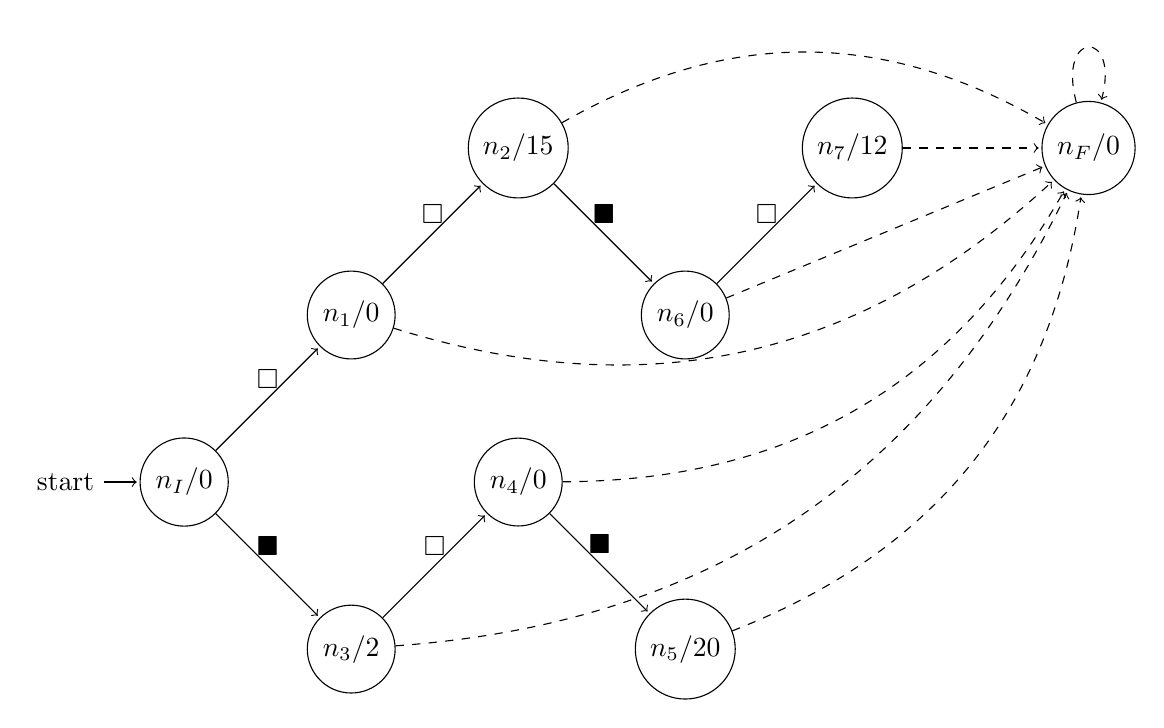
\begin{tikzpicture}[node distance=3cm,on grid,auto,shorten >=1pt]
			\node[initial,state] (0) 				{$n_I/0$};
			\node[state] (1) [above right=of 0]		{$n_1/0$};
			\node[state] (2) [above right=of 1]		{$n_2/15$};
			\node[state] (3) [below right=of 0]      {$n_3/2$};
			\node[state] (4) [above right=of 3]      {$n_4/0$};
			\node[state] (5) [below right=of 4]      {$n_5/20$};
			\node[state] (6) [below right=of 2]      {$n_6/0$};
			\node[state] (7) [above right=of 6]      {$n_7/12$};
			\node[state] (8) [right=of 7]            {$n_F/0$};
			\path[->] 	(0) edge 	node [above] {$\square$}			(1)
							edge    node [above] {$\blacksquare$}	(3)
						(1) edge 	node [above] {$\square$}			(2)
						(2) edge		node [above] {$\blacksquare$}	(6)
						(3) edge    node [above] {$\square$}        	(4)
						(4) edge		node [above] {$\blacksquare$}	(5)
						(6) edge		node [above] {$\square$}			(7)
						;
			\path[->,dashed] (1) edge [bend right]		node {} (8)
							 (2) edge [bend left]		node {} (8)
							 (3) edge [bend right]		node {} (8)
							 (4) edge [bend right]		node {} (8)
							 (5) edge [bend right]		node {} (8)
							 (6) edge		node {} (8)
							 (7) edge 		node {} (8)
							 (8) edge[loop above] node  {}   ();	\end{tikzpicture}
\caption{Final reward controller}
\label{f:final_reward_controller_regex}
\end{figure}

\subsection*{Implementation}
In \href{https://gitlab.science.ru.nl/srietbergen/thesis/-/blob/master/code/reward_controller_seq.py}{\texttt{code/reward\textunderscore controller\textunderscore seq.py}} we have the following:\\

\texttt{reward\textunderscore controller\textunderscore from\textunderscore sequences(sequences,omega)}\\
Given a dictionary in the shape of $\{\texttt{seq}_1 : r_1,\:\texttt{seq}_2 : r_2,\dots,\: \texttt{seq}_n : r_n\}$ together with the set $\Omega$ representing the input alphabet, it will return a reward controller as described in \algorithmref{procedure:into_reward_controller}.

\section{From regular expressions}
\label{sec:rc-regex}

\towrite{introduction into why using regular expressions for rewards}

Given a number of regular expressions over observations defined as $e_1,e_2,\dots,e_n$ together with their respective rewards $r_1,r_2,\dots,r_n\in\mathbb{R}$. Let us define a reward function $R$ that maps the regular expression to their respective reward, in other words $R(e_i)=r_i$. \\

We want to create a reward controller that mimics the behaviour of several regular expressions and their associated rewards. Note that we only want a reward when the sequence of observations is accepted by the language generated by the regular expression. The first step would be is to create a DFA that is generated by the regular expression given. This can be done through simply turning the regular expression into a Non-Deterministic Finite Automaton (with $\lambda$-transitions) and then turning that into a DFA or using other known methods\cite{p:regex-to-dfa}. All that is left for a single regular expression is to keep track of the rewards associated to their final states.\\

So given the $n$ regular expression, we create $n$ DFAs. Let $D_i=(Q_i,q_{0,i},\Omega, \delta_i,F_i)$ be the DFA that accepts the language generated by $e_i$. And then per construction we have that $L(D_i)=L(e_i)$. \\

Note that since we want to obtain a reward controller, we have to encode the reward in the nodes. This is solved by only encoding the reward of DFA $D_i$ in all states of $F_i$. For example if $\texttt{seq}\in\Omega^*$ gets accepted by $D_i$, we have to make sure that the state it ends up in - i.e. the final state(s) - has the reward encoded in its state(s). This is done by the following definition.
\begin{definition}
Let $R_A:Q_1\cup Q_2\cup\dots\cup Q_n\to\mathbb{R}$ be a function that maps any state $q$ of all the state spaces of $D_1,D_2,\dots,D_n$ to their respective rewards. If $q$ is a final state of DFA $D_i$ it should get the reward corresponding to the regular expression used for that specific DFA. In other words,
\begin{equation*}
R_A(q) = \begin{cases}
R(e_i) & \text{ if } q\in F_i \\
0 & \text{ otherwise }
\end{cases}
\end{equation*}
\label{d:associated_reward}
\end{definition}

Having obtained all these seperate DFAs, we can now create a DFA that will accept any word that is accepted by any of the seperate DFAs as follows.

\begin{definition}
The induced product DFA for given DFAs $D_1,D_2,\dots,D_n$ where $D_i=(Q_i,q_{0,i},\Sigma,\delta_i,F_i)$ is a tuple $D=(Q,q_0,\Sigma,\delta,F)$ where 
\begin{itemize}
\item $Q = Q_1 \times Q_2 \times \dots \times Q_n$
\item $q_0 = \langle q_{0,1}, q_{0,2}, \dots, q_{0,n}\rangle$
\item $\Sigma$, the same input alphabet
\item $\delta(\langle q_1,q_2,\dots,q_n\rangle,a)= \langle \delta_1(q_1,a), \delta_2(q_2,a),\dots,\delta_n(q_n,a)\rangle$
\item $F=\{\langle q_1,q_2,\dots,q_n\rangle \mid \exists i \in \{1,2,\dots,n\} : q_i\in F_i\}$
\end{itemize}
\label{d:product_automaton}
\end{definition}

\begin{lemma}
Given $n$ DFAs where $D_i=(Q_i,q_{0,i}, \Sigma,\delta_i,F_i)$, let $D$ be the product automaton as obtained in \defref{d:product_automaton}. Then we $L(D)=L(D_1)\cup L(D_2)\cup \dots L(D_n)$.
\begin{proof}
	\begin{flalign*}
		w\in L(D) &\Longleftrightarrow \delta_N^*(q_0,w)\in F \\
		& \Longleftrightarrow \langle \delta_1^*(q_{0,1},w), \delta_2^*(q_{0,2},w),\dots,\delta_n^*(q_{0,n},w)\rangle\in F \\
		&\Longleftrightarrow \exists i\in\{1,\dots,n\} :  \delta_i^*(q_{0,i},w)\in F_i \\
		&\Longleftrightarrow \delta_1^*(q_{0,1},w)\in F_1 \text{ or } \delta_2^*(q_{0,2},w)\in F_2 \text{ or } \dots \text{ or } \delta_n^*(q_{0,n},w)\in F_n \\
		& \Longleftrightarrow w \in L(D_1) \text{ or } w\in L(D_2) \text{ or } \dots \text{ or } w\in L(D_n)\\
		&\Longleftrightarrow w\in L(D_1)\cup L(D_2)\cup \dots \cup L(D_n)
	\end{flalign*}
\end{proof}
\end{lemma}

The only step left to obtain the reward controller is to connect the obtained product DFA together with the associated rewards of the states.

\begin{definition}
Given a (product) DFA $N=(Q,q_0,\Omega,\delta,F)$ and the associated reward function $R_A$, we define the induced reward controller $\mathcal{F}=(N,n_I,\Omega, \mathbb{R}, \delta_\mathcal{F},\sigma)$ as follows
\begin{itemize}
\item $N=Q$
\item $n_I=q_0$
\item $\delta_\mathcal{F}=\delta$
\item $\sigma: Q\to\mathbb{R}$ where $\sigma(\langle q_1,q_2,\dots, q_n\rangle) = \sum\limits _{i=1}^n R_A(q_i)$
\end{itemize}
\label{d:reward_controller_regex}
\end{definition}

Note that the $\sigma$ is defined by taking the sum over the associated rewards. This is because if we have a sequence $\texttt{seq}\in\Omega^*$ that is accepted by several regular expressions given, it should then obtain all the seperate rewards associated with those regular expressions. Through the following lemma we ensure that for any sequence $\texttt{seq}\in\Omega^*$ the reward controller obtains the combination of rewards depending on the final state after having read $\texttt{seq}$.

\begin{lemma}
Given $e_1,e_2,\dots,e_n$ a sequence of regular expression together with their associated rewards $r_1,r_2,\dots,r_n$, let $D$ be the product automaton as defined in \defref{d:product_automaton} build from the DFAs $D_i$ for which $L(D_i)=L(e_i)$. Then let $\mathcal{F}=(N,n_I,\Omega,\mathbb{R},\delta,\sigma)$ be the reward controller as defined in \defref{d:reward_controller_regex} given $D$. We say that for all possible words $\texttt{seq}\in\Omega^*$ the following holds:
\[\sigma(\delta^*(n_I,\texttt{seq}))=\sum\limits_{e\in\{e_i\mid\texttt{seq}\in L(e)\}}R(e_i)\]
\begin{proof}
\begin{flalign}
\sigma(\delta^*(n_I,\texttt{seq})) &= \sigma(\langle q1,q2,\dots,q_n\rangle)  \label{p:r_l1} \\
	&= \sum\limits_i^n R_A(q_i)\label{p:r_l2}\\
	&= \sum\limits_{\substack{i\in\{1,\dots,n\}\\ q_i\in F_i}} R_A(q_i) \label{p:r_l3}\\
&= \sum\limits_{\substack{i\in\{1,\dots,n\}\\ q_i\in F_i}} R(e_i) \label{p:r_l4}\\
&= \sum\limits_{\substack{i\in\{1,\dots,n\}\\ \delta^*(q_{0,i},\texttt{seq}) \in F_i }} R(e_i)\label{p:r_l5}\\
&= \sum\limits_{\substack{i\in\{1,\dots,n\}\\ \texttt{seq}\in L(D_i)}} R(e_i)\label{p:r_l6}\\
&= \sum\limits_{\substack{i\in\{1,\dots,n\}\\ \texttt{seq}\in L(e_i)}}R(e_i)\label{p:r_l7}\\
&= \sum\limits_{e\in\{e_i\mid\texttt{seq}\in L(e_i)\}} R(e)\label{p:r_l8}
\end{flalign}
For \equref{p:r_l1} we simply use \defref{d:delta_star_rc} and the fact that $D$ is deterministic, so it ends up in an unique state after reading $\texttt{seq}$.
For \equref{p:r_l2} we use the definition for $\sigma$ as seen in \defref{d:reward_controller_regex}. For \equref{p:r_l3} we use that fact that in \defref{d:associated_reward} we observe that $R_A(q_i)$ is equal to zero if $q_i\notin F_i$ and only produces a non-zero value for all $q_i\in F_i$. Thus we only look at the $q_i$ which return a non-zero value. Since we now know we only look at the non-zero reward values, we can use \defref{d:associated_reward} again in \equref{p:r_l4}. From \defref{d:delta_star} we can rewrite the equation in \equref{p:r_l5}. For \equref{p:r_l6} we use \defref{d:accepted_language}. Since per construction $L(e_i)=L(D_i)$ for all $i\in\{1,\dots,n\}$, we rewrite the term in \equref{p:r_l7}. Finally in \equref{p:r_l8} we simply rewrite the term under the sum.
\end{proof}
\label{lem:proof_regex}
\end{lemma}

Logically, the size of the reward controller obtained through a series of $n$ automata is bounded by $|D_1||D_2| \dots  |D_n|$, where $D_i$ is the automata obtained through the regular expressions $e_i$. When implementing this, make sure to minimize the automata whenever possible to decrease the sizing of the reward controller. \todo{implementation relevant?}

\subsection*{Example}
Let's say we are given 2 regular expressions. One is that an even number off $\square$ gives a reward of $10$ and the other states that an odd number of $\blacksquare$ gives a reward of $15$. In other words 
$R(e_1)=R(\texttt{even number of }\square)=10$ and $R(e_2)=R(\texttt{odd number of }\blacksquare)=15$\\

Let us first obtain the two DFAs that are generated by $e_1$ and $e_2$. Those can be seen in \figureref{f:e1_e2}. 
\begin{figure}[H]

\begin{subfigure}[H]{0.4\textwidth}
	\centering
		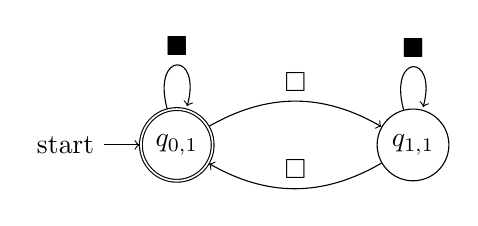
\begin{tikzpicture}[node distance=3cm,on grid,auto]
			\node[initial,state,accepting] (1) 				{$q_{0,1}$};
			\node[state] (2) [right=of 1]		{$q_{1,1}$};
			\path[->] 	(1) edge[bend left] 	node [above] {$\square$}			(2)
							edge[loop above] node [above] {$\blacksquare$}   ()
						(2) edge[bend left] 	node [above] {$\square$}			(1)
							edge[loop above] node [above] {$\blacksquare$}   ();
	\end{tikzpicture}
\caption{DFA for regular expression even number of $\square$}
\end{subfigure}
\hfill
\begin{subfigure}[H]{0.4\textwidth}
	\centering
		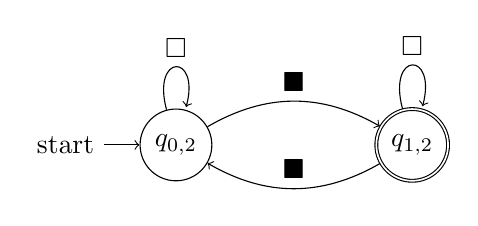
\begin{tikzpicture}[node distance=3cm,on grid,auto]
			\node[initial,state] (1) 				{$q_{0,2}$};
			\node[state,accepting] (2) [right=of 1]		{$q_{1,2}$};
			\path[->] 	(1) edge[bend left] 	node [above] {$\blacksquare$}			(2)
							edge[loop above] node [above] {$\square$}   ()
						(2) edge[bend left] 	node [above] {$\blacksquare$}			(1)
							edge[loop above] node [above] {$\square$}   ();
	\end{tikzpicture}
\caption{DFA for regular expression for odd number of $\blacksquare$}
\end{subfigure}
\caption{}
\label{f:e1_e2}
\end{figure}
Then we create the product automaton as defined in \defref{d:product_automaton}. The result can be seen in \figureref{f:pd}. 

\begin{figure}[H]
	\centering
		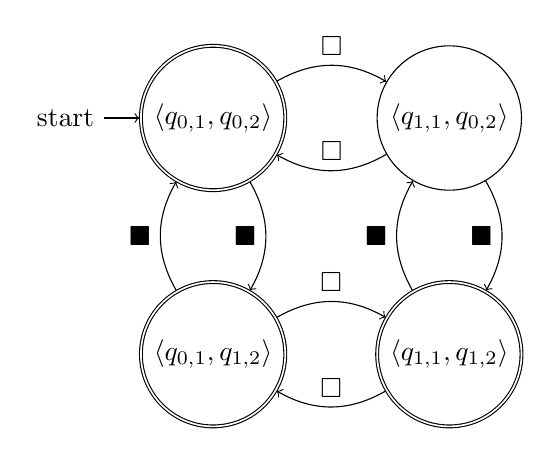
\begin{tikzpicture}[node distance=3cm,on grid,auto]
			\node[initial,state,accepting] (1) 				{$\langle q_{0,1}, q_{0,2} \rangle$};
			\node[state] (2) [right=of 1]		{$\langle q_{1,1}, q_{0,2} \rangle$};
			\node[state,accepting] (3) [below=of 1]		{$\langle q_{0,1}, q_{1,2} \rangle$};
			\node[state,accepting] (4) [right=of 3]		{$\langle q_{1,1}, q_{1,2} \rangle$};
			\path[->] 	(1) edge[bend left] 	node [above] {$\square$}			(2)
							edge[bend left] 	node [left] {$\blacksquare$}			(3)
						(2) edge[bend left] 	node [above] {$\square$}			(1)
							edge[bend left] 	node [left] {$\blacksquare$}			(4)
						(3) edge[bend left] 	node [left] {$\blacksquare$}			(1)
							edge[bend left] 	node [above] {$\square$}			(4)
						(4) edge[bend left] 	node [left] {$\blacksquare$}			(2)
							edge[bend left] 	node [above] {$\square$}			(3);
	\end{tikzpicture}
\caption{Product DFA for both regular expressions}
	\label{f:pd}
\end{figure}

From this we then obtain the reward controller as per \defref{d:reward_controller_regex}, and can be found in \figureref{f:rc}. Note that 
\begin{flalign*}
R_A(q_{0,1})&=10\\
R_A(q_{1,1})&= R_A(q_{0,2})=0\\
R_A(q_{1,2})&=15
\end{flalign*}

\begin{figure}[H]
	\centering
		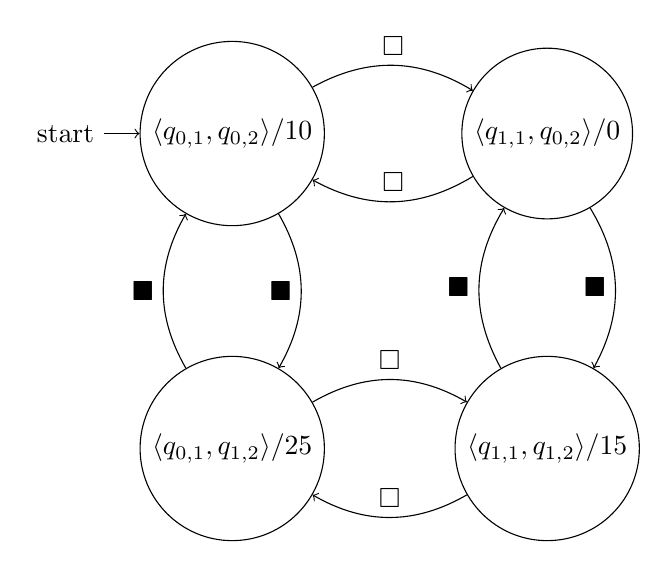
\begin{tikzpicture}[node distance=4cm,on grid,auto]
			\node[initial,state] (1) 			{$\langle q_{0,1}, q_{0,2} \rangle /10$};
			\node[state] (2) [right=of 1]		{$\langle q_{1,1}, q_{0,2} \rangle /0$};
			\node[state] (3) [below=of 1]		{$\langle q_{0,1}, q_{1,2} \rangle /25$};
			\node[state] (4) [right=of 3]		{$\langle q_{1,1}, q_{1,2} \rangle /15$};
			\path[->] 	(1) edge[bend left] 	node [above] {$\square$}			(2)
							edge[bend left] 	node [left] {$\blacksquare$}			(3)
						(2) edge[bend left] 	node [above] {$\square$}			(1)
							edge[bend left] 	node [left] {$\blacksquare$}			(4)
						(3) edge[bend left] 	node [left] {$\blacksquare$}			(1)
							edge[bend left] 	node [above] {$\square$}			(4)
						(4) edge[bend left] 	node [left] {$\blacksquare$}			(2)
							edge[bend left] 	node [above] {$\square$}			(3);
	\end{tikzpicture}
\caption{Reward Controller for $R$}
	\label{f:rc}
\end{figure}

\subsection*{Implementation}
We used \cite{g:regex-to-dfa} as a base for creating a DFA from a given regular expression. The regular expression needs to have the following grammar (this can also be seen in \texttt{code/regex-to-dfa/grammar/RegEx.g4}):
\begin{alltt}
prog : (regex newline)*;

regex : regex '*'      #kleene-star
  | regex regex	       #concatenation
  | regex '|' regex    #alternation
  | ID         	       #identifier
  | '\(\lambda\)'	   #epsilon
  | '(' regex ')'      #parenthesis
  ;

newline : '\(\backslash\)n{}';

ID: [a-zA-Z0-9];
WS: [\(\backslash\)t\(\backslash\)r ]->skip;
\end{alltt}

In \href{https://gitlab.science.ru.nl/srietbergen/thesis/-/blob/master/code/reward_controller_regex.py}{\texttt{code/reward\textunderscore controller\textunderscore regex.py}} we have the following:\\

\texttt{rename(D)}\\
Transform the given reward controller $D$ into one that ensures that the states are labeled with numbers from $0$ to $|D|-1$. \\

\texttt{regex\textunderscore to\textunderscore dfa(regex, omega)}:\\
Given a regular expression conform to the syntax as defined above and the input language $\Omega$ over which it is defined, we transform it into a DFA.\\

\texttt{union(machines, rewards)}:\\
Given a list $n$ of \texttt{machines} ($D_1,D_2,\dots, D_n$) and a list or $n$ rewards ($r_1,r_2,\dots, r_n$), we create the induced product DFA according to \defref{d:product_automaton}. Then we (create and) return the induced reward controller as defined in \defref{d:reward_controller_regex}.\\

\texttt{reward\textunderscore controller\textunderscore from\textunderscore regex(info,omega):}:\\
Given $n$ regular expressions together with their associated reward in dictionary ($\{e_1 :r_1, e_2:r_2, \dots e_n:r_n\}$), together with the input language $\Omega$ specified, we return the reward controller representing the information given. 


	
	\chapter{Obtaining policy}
	\towrite{introduction}
%add extra final state, in which we encode the actual transitions, the end state will be used to marked you are done. 

\begin{definition}
	\label{def:reward-mdp}
	The induced POMDP for reward controller $\mathcal{F}=(N, n_I, \Omega, \mathcal{R}, \delta, \lambda)$ on a POMDP $\mathcal{M}=(M,\Omega,Obs)$ where $M=(S,s_I,A,T_{M})$ is a tuple $\mathcal{M'}=(M',\Omega',Obs')$ where 
	\begin{itemize}
		\item $M' = (S',s'_I,A',T_{M'},\mathcal{R})$, the hidden MDP defined as follows
		\begin{itemize}
			\item $S'=S\times N \cup \{s_F\}$
			\item $s'_I = \langle s_I, \delta(n_I, O(s_I))\rangle$
			\item $A'=A\cup \{\texttt{end}\}$
			\item $T_{M'}:S'\times A \to \Pi(S)$ where
				\begin{align*}
					T_{M'}(\langle s,n\rangle,a,\langle s',n'\rangle) &= \begin{cases}
						T_M(s,a,s') & \text{if } \delta(n,O(s')=n') \\
						0 & \text{otherwise}
					\end{cases}\\
					T_{M'}(s,\texttt{end},s_F) &= 1 \text{ for all} s\in S'
				\end{align*}
			\item $R:S'\times A'\times S' \to \mathcal{R}$ where 
                \begin{align*}
					R(s',\texttt{end},s_F) &= 
					\begin{cases}
						\sigma(n) & \text{ if } s'=\langle s,n\rangle \\
						0         & \text{ if } s'=s_F
					\end{cases}
					\\
					R(s,a,s') &= 0 \text{ for all } s'\in S'\setminus \{s_F\}
				\end{align*}
		\end{itemize}
		\item $\Omega'=\Omega \cup \{o_F\}$, the observation state
		\item $Obs:S'\to \Omega'$ where 
			\begin{equation*}
				Obs'(s)= \begin{cases}
				Obs(s') & \text{if } s=\langle s',n\rangle\\
				o_F & \text{if } s=s_F
				\end{cases}
			\end{equation*}
		\end{itemize}
\end{definition}



	
	
	%\chapter{Belief-based Rewards}
	%\section{Partially Observable MDPs}
Partially Observable Markov Decision Processes have been used to model problems
concerning sequential decision-making where the model is uncertain. The objective is
to act in a way that optimizes a performance criterion. This often translates itself to
maximizing a certain reward, or minimizing certain costs involved.

\subsection{Definitions}

\begin{definition}[Partially Observable Markov Decision Process]
	A Partially Observable Markov Decision Process, or POMDP, is a tuple $(S, \mathcal{A}, \Omega, T, O, r, b_0)$, where
	\begin{itemize}
		\item $S$, the state space;
		\item $A$, the action space;
		\item $\Omega$, the observation space;
		\item $T:S\times \mathcal{A} \times S \to [0,1]$, the transition function where
			$T(s,a,s')=Pr(s'\mid s,a)$;
		\item $O:S\times \mathcal{A} \times \Omega \to [0,1]$, the observation function where
		$O(s',a,o)= Pr(o\mid s',a)$
		\item $r: S \times \mathcal{A} \to \mathds{R}$, the reward function, and 
		\item $b_0 : S \to [0,1]$, the initial probability distribution over states.
	\end{itemize}
\end{definition}

A POMDP is only partially observable, which indicates that we do not know everything about the model. We specifically are unaware of what state a POMDP currently is in. To create a notion of what state we believe to be in, we use belief states.

\begin{definition}[Belief state]
	Given a POMDP $(S, \mathcal{A}, \Omega, T, O, r, b_0)$, a belief state $b$ is a probability distribution over $S$ called $\Delta$. The probability of the POMDP being in state $s$ according to belief $b$, is denoted by $b(s)$. Logically $\sum_{s\in S}b(s)=1$ and for all states $s$ we have that $b(s)\in[0,1]$.
\end{definition}

A belief state evolves over time and a POMDP will start in their initial belief state $b_0$.
The belief state will be updates according to the action that is undertaken and an observation that will be observed after taking said action.

\begin{definition}[Updated belief state]
Let $Pr(o|a,b)=\sum_{s,s'\in S}O(s'',a,o)T(s,a,s'')b(s)$. The probability of ending in state $s'$ after performing an action $a$ and then observing observation $o$ is calculated as
\begin{equation*}
	b^{a,o}(s')=\frac{O(s,a,o)}{Pr(o | a,b)}\sum_{s\in S} T(s,a,s')b(s)
\end{equation*}
\end{definition}

With the help of belief states, we can create a fully observable continuous space belief MDP representing a POMDP.

\begin{definition}[Belief MDP]
	A POMDP $(S, A, \Omega, T, O, r, b_0)$ can be written as a belief MDP $(\Delta, \mathcal{A}, \tau, \rho)$, where
	\begin{itemize}
		\item $\Delta = \Pi(S)$, the set of probability distributions over S;
		\item $\mathcal{A}$, the action space;
		\item $\tau : \Delta \times \mathcal{A} \times \Delta \to [0,1]$, the new transition function
		\item $\rho: \Delta \times \mathcal{A} \to \mathds{R}$, the new reward function.
	\end{itemize}
\end{definition}

The objective is to maximize the expected cumulative reward, which is done by looking for an optimal policy. Let $\gamma$ be some discount factor and $\rho_t$ be the expected immediate reward obtained at a certain step $t$, then the expected cumulative reward is defined as

\begin{equation*}
	J^\pi(b)=E \big[\sum_{t=0}^{\infty}\gamma \rho_t\mid b,\pi\big]
\end{equation*}

With this information, we can calculate the optimal policy 
\begin{equation}
\pi^* = \argmax_{\pi\in \mathcal{A}^\Delta} J^\pi(b_0)
\end{equation}

The value $J^{\pi^*}(b_0)$ can be computed recursively through a value function $V_n$, due to Bellman's principle of optimality\cite{p:bellman}. If we let $H$ be the possible infinite horizon of the problem, the optimal value can be concluded from $J^{\pi^*}(b)=V_{n=H}(b)$.

\begin{definition}[Value function for POMDPs]
For $b\in\Delta$, let the value function be defined as
\begin{flalign}
	V_0(b) & = 0 \nonumber \\
	V_n(b) & = \max_{a\in \mathcal{A}}\big[\rho(b,a) + \gamma\int_{\Delta}\tau(b,a,b')V_{n-1}(b')db'\big] \nonumber \\
	\label{eqn:value_fun}
	&= \max_{a\in \mathcal{A}} \big[\rho(b,a) + \gamma\sum_{o\in\Omega} Pr(o\mid a, b) V_{n-1}(b^{a,o}) \big] 
\end{flalign}
\end{definition}

Observe that the reward function for a POMDP is based on a state and action through $r(s,a)$, while the reward function for a belief MDP depends on the belief state and action through $\rho(b,a)$. The belief MDP reward function $\rho$ can be derived from the POMDP reward function $r$ like so
\begin{equation}
	\label{eqn:reward_belief_mdp}
	\rho(b,a)=\sum_{s\in S}b(s)r(s,a)
\end{equation}

When the $\rho$ is defined as in Equation~\ref{eqn:reward_belief_mdp}, the recursive computation in Equation~\ref{eqn:value_fun} has the property to generate piecewise-linear and convex (PWLC) value functions for each horizon\cite{p:pwlc}.  

\begin{definition}[Piecewise-linear function]
	A function is piecewise-linear if it consists of $n$ linear segments defined over $n$ intervals.
\end{definition}

\begin{definition}[Convex function]
	A function $f:A\to B$ is convex if for all $\theta\in[0,1]$ and $x_1,x_2\in A$
	\begin{equation*}
		f(\theta x_1 + (1-\theta) x_2)\leq \theta f(x_1) + (1-\theta)f(x_2)
	\end{equation*}
\end{definition}

For example, if we claim that $\Gamma_n$ is the set of vectors representing the value function for horizon $n$, we can rewrite the value function to $V_n(b)=\max_{\alpha\in\Gamma_n}\sum_{s\in S} b(s)\alpha(s)$. 

\subsection{Solving with exact updates}
Using the PWLC property, Equation~\ref{eqn:value_fun} can be refactored to be able to perform the Bellman update. Let $\chi_n(b,s)=(\chi_n(b))(s)$ where $\chi_n(b)=\argmax_{\alpha\in \Gamma_n} b\cdot\alpha$, so $\chi_n(b)$ returns the hyperplane that is maximal for a given belief state $b$. The refactored value function is then written as 

\begin{equation}
	V_n(b) = \max_{a\in \mathcal{A}}\sum_{o\in \Omega}\sum_{s\in S}b(s)\big[\frac{r(s,a)}{|\Omega|} + \sum_{s'\in S}T(s,a,s')O(s',a,o)\chi_{n-1}(b^{a,o},s')\big]
\end{equation}

Let’s solely look at the terms within in the brackets. They are dependent on a certain action and observation. So for a given $o\in\Omega, a\in\mathcal{A}$, the set of $\alpha$-vectors is generated by $\overline{\Gamma_n}^{a,o}$. Let $r^a(s)=r(s,a)$ and $P^{a,o}(s,s')=T(s,a,s')O(s',a,o)$ in 
\begin{equation}
	\overline{\Gamma_n}^{a,o}=\{ \frac{r^a}{|\Omega|}+P^{a,o}\cdot\alpha_{n-1}\mid\alpha_{n-1}\in\Gamma_{n-1} \}
\end{equation}

Observe that there are $|\mathcal{A}|\times|\Omega|$ of such $\overline{\Gamma_n}^{a,o}$ sets. To create the set containing all
of these possible observation and action combination we take the following cross-sum:
\begin{equation}
	\overline{\Gamma_n} = \bigcup_{a\in\mathcal{A}}\bigoplus_{o\in \Omega}\overline{\Gamma_n}^{a,o}
\end{equation}
Note that the operator $\oplus$ is defined as $U \oplus W = \{u + w | u \in U, w \in W\}$.\\

Since $\overline{\Gamma_n}$ is created through all possible combination, it also contains $\alpha$-vectors that are useless because the corresponding hyperplanes are below the value function. To create the actual $\Gamma_n$ set from $\overline{\Gamma_n}$, we can use one of several pruning techniques on the $\overline{\Gamma_n}$ set which will get rid of the dominating useless vectors.

\section{Extension for Active Sensing}

All problems who only have partial observability tackle a certain issue through getting information about the model or achieving some goal. Most of the time, the concerning problem is tackled through obtaining enough information get an optimal reward. However, some \textit{active sensing} problems (where the objective is acting in a way to acquire knowledge about a part of the model or minimizing the entropy over a given state
variable) cannot be resolved this way. For these problems, the performance of an agent should incorporate their obtained knowledge of the system thus far. \\

In Equation~\ref{eqn:reward_belief_mdp}, we observe that the reward of a POMDP is solely based on the current state and action. We want the agent to include their obtained knowledge, but simply putting the entire history of the model in the state, would lead to a combinatorial explosion. \\

To tackle this issue, we propose a new method of defining rewards based on the acquired knowledge through the usage of belief states. Since we will use a different definition than the one described in Equation~\ref{eqn:reward_belief_mdp}, the direct link with POMDPs is broken. Luckily, a lot of the components of a POMDP are still usable. For this we use a generalization of the POMDP framework, where the reward is directly defined as a function $\rho(b,a)$.

\subsection{Definitions}
\begin{definition}[$\rho$POMDP]
	A $\rho-$based POMDP ($\rho$POMDP) is a tuple $(S,\mathcal{A},T,O,\rho,b_0)$, where
		\begin{itemize}
		\item $S$, the state space;
		\item $A$, the action space;
		\item $\Omega$, the observation space;
		\item $T:S\times \mathcal{A} \times S \to [0,1]$, the transition function where
		$T(s,a,s')=Pr(s'\mid s,a)$;
		\item $O:S\times \mathcal{A} \times \Omega \to [0,1]$, the observation function where
		$O(s',a,o)= Pr(o\mid s',a)$;
		\item $\rho: \Delta \times \mathcal{A} \to \mathds{R}$, the reward function, and ;
		\item $b_0 : S \to [0,1]$, the initial probability distribution over states.
	\end{itemize}
\end{definition}

We see that $\rho$ is often just some uncertainty or error measure, but it can also be combined with some expected state-reward.

\subsection{Convexity property}

Observe that the belief-based value function for POMDPs is convex (Equation~\ref{eqn:value_fun}), because $r(s,a)$ is linear in Equation~\ref{eqn:reward_belief_mdp}. The value function for $\rho$-POMDPs is also convex, if $/rho(b,a)$ is convex.

\begin{theorem}
	If $\rho$ and $V_0$ are convex functions over $\delta$, then the value function $V_n$ of the belief MDP is convex over $\Delta$ at any time step $n$.
\end{theorem}

Note that $\rho(b,a)$ being convex over $\Delta$ is due to the fact that uncertainty measures are naturally convex\cite{p:belief-dependent-rewards}. We will only be focusing on reward functions that are convex. The initial value function $V_0=0$ for finite-horizon problems, but can be any convex function for infinite-horizon problems.

\subsection{Solving with exact updates}
We assume that this belief-based $\rho$ is a PWLC function. Therefore it can be represented as several $\Gamma$-sets; one $\Gamma^a_\rho$ for each action in $\mathcal{A}$:
\begin{equation}
	\label{eqn:reward_belief}
	\rho(b,a)=\max_{\alpha\in\Gamma^a_\rho}\big[\sum_{s}b(s)\alpha(s)\big]
\end{equation}

We now rewrite the value function from Equation~\ref{eqn:value_fun} together with the new reward
function from Equation~\ref{eqn:reward_belief}. Let $\chi_\rho^a(b,s) = (\chi_\rho^a(b))(s)$ where $\chi_\rho^a(b)=\argmax_{\alpha\in\Gamma^a_\rho}(b\cdot\alpha)$. The rewritten value function for $\rho$POMDPs is then
\begin{equation}
	V_n(b)= \max_{a\in \mathcal{A}}\sum_{s\in S}b(s) \big[\chi_\rho^a(b,s) + \sum_{o\in \Omega}\sum_{s'\in S}T(s,a,s')O(s',a,o)\chi_{n-1}(b^{a,o},s') \big]
\end{equation}

This new value function makes use of $\Gamma_\rho^a$ through $\chi_\rho^a$, but also generates $|\mathcal{A}|\times|\Omega|$ $\Gamma$-sets called $\overline{\Gamma_n}^{a,o}$, where $P^{a,o}(s,s')=T(s,a,s')O(s',a,o)$, defined as:
\begin{equation}
	\overline{\Gamma_n}^{a,o}=\{P^{a,o}\cdot\alpha_{n-1}\mid\alpha_{n-1}\in\Gamma_{n-1}\}
\end{equation}

Just like for POMDPs, we can use exact algorithms for $\rho$POMDPs. The difference is that now the cross-sum to calculate $\overline{\Gamma_n}$ now includes 
\begin{itemize}
	\item one $\alpha^{a,o}$ for each observation $\Gamma$-set $\overline{\Gamma_n}^{a,o}$, and
	\item one $\alpha_\rho$ from the $\Gamma$-set $\Gamma_\rho^a$ corresponding to the reward.
\end{itemize}
This results in the new cross-sum 
\begin{equation}
	\overline{\Gamma_n}=\bigcup_{a\in\mathcal{A}}\big[\bigoplus_{o\in \Omega}\overline{\Gamma_n}^{a,o}\oplus\Gamma_\rho^a\big]
\end{equation}

The number of vectors that are being generated is larger than for a regular POMDP. Let $|R|$ be the number of $\alpha$-vectors specifying the $\rho(b,a)$ function, which depends on the action that was taken. The total amount of vectors is thus $|R| \times |\mathcal{A}| × |\Omega|$.
	
	%\chapter{Finite State Controllers}
	%\section{Definitions}

\begin{definition}[Parametric MDP]
 $M=(S,s_I,\mathcal{A},V,\mathcal{P})$ where
 \begin{itemize}
 	\item $S$, the state space;
 	\item $s_I$, the initial state;
 	\item $\mathcal{A}$, the action space;
 	\item $V$, the parameter space;
 	\item $\mathcal{P}:S\times \mathcal{A} \times S \to \mathbb{Q}[V]$, the transition function.
 	\towrite{polynomial notation and stuff}
 \end{itemize}
\end{definition}

Let $A(s)$ denote the available actions, i.e. $A(s)=\{a\in \mathcal{A} \mid \exists s'\in S: \mathcal{P}(s,a,s')\neq 0 \}.$

\begin{definition}[MDP]
	A MDP is a pMDP where 
	\begin{itemize}
		\item $\mathcal{P}:S\times\mathcal{A}\times S \to [0,1]\subseteq\mathbb{R}$
		\item for all states $s\in S, a\in\mathcal{A},\sum_{s'\in S}\mathcal{P}(s,a,s')=1$
	\end{itemize}
\end{definition}

\begin{definition}[pMC]
	A (parametric) Markov Chain is a (parametric) MDP where $|A(s)|=1$ for all $s\in S$.  Usually denoted as $D=(S,s_I,V,\mathcal{P})$, where $\mathcal{P}:S\times S\to \mathbb{Q}[V]$ because the actions are irrelevant. 
\end{definition}


\begin{definition}[Strategy]
	A strategy $\sigma$ for a (p)MDP is a function that takes a finite path corresponding to $M$ and returns a distribution over actions, $\sigma:\text{Paths}^M_{fin}\to \Pi(\mathcal{A})$. These strategies need to comply with $supp(\sigma(\pi))\subseteq A(last(\pi))$.
\end{definition}
\towrite{last, pi notation of paths, and supp}

\begin{definition}[POMDP]
	A POMDP $\mathcal{M}$ can also be seen as a tuple $(M,\Omega,Obs)$ where
	\begin{itemize}
		\item $M=(S,s_I,\mathcal{A},\mathcal{P})$, the underlying MDP;
		\item $\Omega$, the finite set of observations;
		\item $Obs: S\to\Omega$, the observation function.
	\end{itemize}
\end{definition}

If for all states $s,s'\in S: Obs(s)=Obs(s')$, then $A(s)=A(s')$.
If $O(s)=z$, then $A(z)=A(s)$.

\begin{definition}[Observation-based Strategy]
	An observation-based strategy is $\sigma:\text{Paths}^M_{fin}\to \Pi(\mathcal{A})$ for an underlying MDP $M$ such that if for all paths $\pi,\pi'\in\text{Paths}^M_{fin}$ where $Obs(\pi)=Obs(\pi')$ we claim that $\omega(\pi)=\omega(\pi')$.
\end{definition}

\begin{definition}[Finite State Controller]
	FSC $F=(N,n_I,\gamma,\delta)$ where
	\begin{itemize}
		\item $N$, the set of memory nodes
		\item $n_I$, the initial memory node
		\item $\gamma:N\times \Omega \to \Pi(\mathcal{A})$, the action mapping
		\item $\delta:N\times \Omega \to \mathcal{A} \to \Pi(N)$, the memory update. 
	\end{itemize}
\end{definition}
	

\section{Modelling MDPs with FSC}

\section{Modelling POMDPs with FSC}

\section{Belief-based Rewards}
	%\chapter{test}
\section{Domains}
Let's start with the following definition:
\begin{definition}\label{def:domain}
	A set $U \subseteq \mathbb{C}$ is a \emph{domain} if:
	\begin{itemize}
		\item $U$ is open in $\mathbb{C}$, and
		\item $U$ is connected.
	\end{itemize}
\end{definition}


\section{Yumyumyumyum}
\towrite{an introduction and some examples}

\begin{theorem}[]
	Suppose $n \in \mathbb{Z}$, then the following are equivalent:
	\begin{enumerate}[label=\roman*.]
		\item $n > 5$.
		\item $5 > 5$.\todo{This doesn't seem right...}
		\item For each $n \in n$, we have:
		\begin{align}\label{eq:truth}
			n > n+1 > n+1^2 > \dots > n+7.
		\end{align}
		where $7$ is an arbitrary element of
		\begin{align*}
			\oint_{a}^{b} \supersine \alpha + i \supercosine \beta  db(a).
		\end{align*}
	\end{enumerate}
\end{theorem}

\begin{remark}
	Interesting!
\end{remark}
\begin{proof}
	See \cite{NIPS2010_3971}.
\end{proof}

\begin{figure}[h]
	\centering
	\includegraphics[width=.3\textwidth]{img/in_dei_nomine_feliciter.eps}
	\caption{Motivational illustration. Similar to \cite{NIPS2010_3971}.}
	\label{fig:logo}
\end{figure}

\begin{corollary}
	Suppose $U \subseteq \mathbb{C}$ is a domain (see Definition \ref{def:domain}), and $f: \overline{U} \rightarrow \mathbb{C}$ is continuous on $\overline{U}$ and holomorphic on $U$. If $z \mapsto |f(z)|$ is constant on $\partial U$, then $f$ has a zero in $U$.
\end{corollary}
\begin{proof}
	If not, consider $\frac{1}{f}$.
\end{proof}
The proof of this theorem is illustrated in Figure

	
	

	\newpage
	
	% You can choose a citation style, 'plain' is the default
	% See:
	% https://www.overleaf.com/learn/latex/Bibtex_bibliography_styles
	
	\bibliographystyle{plain}
	\bibliography{references}
	
\end{document}

